% Course Exam Style
% By: Hamid Zarrabi-Zadeh
% Licenced Under GPL

\documentclass[11pt,a4paper]{article}

\usepackage{graphicx,comment,framed}
\usepackage{amsthm,amssymb,amsmath}
\usepackage{enumitem}
%\usepackage[colorlinks,linkcolor=blue,citecolor=blue]{hyperref}

\usepackage[localise=on, extrafootnotefeatures]{xepersian}
\usepackage[noend]{algpseudocode}


%--------------------- page settings ----------------------

\settextfont[Scale=1.1]{XB Niloofar}
\setdigitfont[Scale=1.1]{XB Niloofar}
%\defpersianfont\sayeh[Scale=1.1]{XB Kayhan Pook}
\addtolength{\textheight}{3.2cm}
\addtolength{\topmargin}{-24mm}
\addtolength{\textwidth}{3cm}
\addtolength{\oddsidemargin}{-1.5cm}

\renewcommand{\labelitemi}{$\small\bullet$}
\renewcommand{\arraystretch}{1.3}


%------------------------ Environments ------------------------------------

\newtheorem{قضیه}{قضیه}
\newtheorem{لم}{لم}
\newtheorem{مشاهده}{مشاهده}
\newtheorem{تعریف}{تعریف}


%-------------------------- Notations ------------------------------------

\newcommand{\IR}{\ensuremath{\mathbb{R}}} 
\newcommand{\IZ}{\ensuremath{\mathbb{Z}}} 
\newcommand{\IN}{\ensuremath{\mathbb{N}}} 
\newcommand{\IS}{\ensuremath{\mathbb{S}}} 
\newcommand{\IC}{\ensuremath{\mathbb{C}}} 
\newcommand{\IB}{\ensuremath{\mathbb{B}}} 

\newcommand{\bR}{\mathbb{R}}
\newcommand{\cB}{\mathcal{B}}
\newcommand{\cO}{\mathcal{O}}
\newcommand{\cG}{\mathcal{G}}
\newcommand{\rM}{\mathrm{M}}
\newcommand{\rC}{\mathrm{C}}
\newcommand{\rV}{\mathrm{V}}

\newcommand{\ceil}[1]{{\left\lceil{#1}\right\rceil}}
\newcommand{\floor}[1]{{\left\lfloor{#1}\right\rfloor}}
\newcommand{\prob}[1]{{\mbox{\tt Pr}[#1]}}
\newcommand{\set}[1]{{\{ #1 \}}}
\newcommand{\seq}[1]{{\left< #1 \right>}}
\newcommand{\provided}{\,|\,}
\newcommand{\poly}{\mbox{\rm poly}}
\newcommand{\polylog}{\mbox{\rm \scriptsize polylog}\,}
\newcommand{\divs}{\ | \ }
\newcommand{\congruent}[1]{\,\overset{#1}{\equiv}\,}

\newcommand{\lee}{\leqslant}
\newcommand{\gee}{\geqslant}
\renewcommand{\leq}{\lee}
\renewcommand{\le}{\lee}
\renewcommand{\geq}{\gee}
\renewcommand{\ge}{\gee}

\newcommand{\REM}[1]{}
\renewcommand{\حذف}{\REM}
\newcommand{\mrbox}[1]{\mbox{\lr{#1}}}

\newcommand{\لر}{\lr}


\newcounter{probcnt}
\newcommand{\مسئله}[1]{\stepcounter{probcnt}\bigskip\bigskip{
 	\large \bf مسئله‌ی \arabic{probcnt}$\mbox{\bf{.}}$ \ #1} \bigskip}

\newcommand{\fqed}[1]{\leavevmode\unskip\nobreak\quad\hspace*{\fill}{\ensuremath{#1}}}

\newenvironment{اثبات}
	{\begin{trivlist}\item[\hskip\labelsep{\em اثبات.}]}
	{\fqed{\square}\end{trivlist}}

\newenvironment{حل}
	{\begin{trivlist}\item[\hskip\labelsep{\bf حل.}]}
	{\fqed{\blacktriangleright}\end{trivlist}}

\ifdefined\hidesols
	\newsavebox{\trashcan} % uncomment the following line to hide solutions
	\renewenvironment{حل}{\begin{latin}\begin{lrbox}{\trashcan}}{\end{lrbox}\end{latin}}
\fi


%------------------------- Header -----------------------------

\newcommand{\سربرگ}[3]{
\parindent=0em

\rightline{
\makebox[5em][c]{
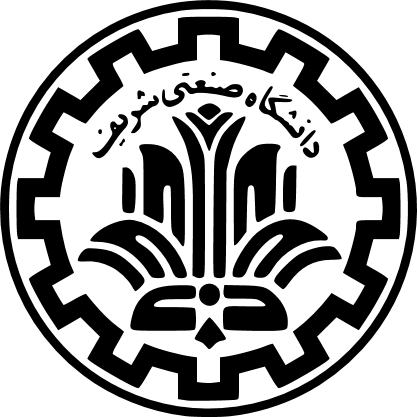
\includegraphics[height=1.5cm]{../commons/sharif.png}
}}
\vspace{-.2em}
{\scriptsize\bf دانشکده‌ی مهندسی کامپیوتر}
\hfill {\small
مدرس:  آبام-بهرامی \  
}\\[-5em]
\leftline{\hfill\large\bf 
ساختمان‌داده‌ها و الگوریتم‌ها
}\\[.2em]
\leftline{\hfill\bf 
نیم‌سال اول ۰۲-۰۳
}\\[1.4em]
\hrule height .12em

\small
\vspace{1mm} 
نام و نام خانوادگی:
\hfill #2 %[2mm]
%شماره‌ی دانش‌جویی:
%\hfill  زمان: #3
%\vspace{1.5mm} 
\hrule height .1em

\vspace{-5.7em} 
\hfill {\large #1} \hfill
\vspace*{4em}
}

\newcommand{\نام‌دانش‌جو}[2]{
\begin{framed}
نام دانش‌جو: #1\hfill شماره‌ی دانش‌جویی: #2
\end{framed}
}

\pagestyle{empty} 



\شروع{نوشتار}

\سربرگ{آزمون میان‌ترم دوم}{۵ دی ۱۴۰۲}{۱۵۰ دقیقه}
\medskip


\مسئله{میانگان} [۱۵ نمره]

 آرایه $A$  شامل $n$ عدد مختلف است. حال می‌خواهیم آرایه $B$ را به این صورت پر کنیم که به ازای هر $i$، $B[i]$ برابر با میانه‌ی اعداد $A[1]$  تا $A[i]$  باشد. الگوریتمی از مرتبه‌ی $O(n\log n)$ برای این مسئله ارائه دهید.

\مسئله{چرخش و توازن}[۲۵ نمره]

در مورد درخت قرمز و سیاه به سوالات زیر پاسخ دهید.
\شروع{شمارش}[label=(\alph*)]
\فقره آیا می‌توان گره‌های هر درخت دودویی جست‌وجویی که ارتفاع آن حداکثر $2\log{n}$ است را با رنگ‌های قرمز و سیاه و طبق قواعد درخت قرمز و سیاه رنگ‌آمیزی کرد؟ (۵ نمره)
\فقره نشان دهید با عمل‌های چرخش به راست و چرخش به چپ می‌توان هر درخت دودویی جست‌وجویی را به هر درخت دودویی جست‌وجوی دیگری تبدیل کرد. (۱۰ نمره)
\فقره برای مسئله‌ی بخش قبل، الگوریتمی ارائه دهید که با حداکثر 
$\mathcal{O}(n\log{n})$  چرخش تبدیل را انجام دهد. 
(۱۰ نمره)
\پایان{شمارش}

\مسئله{درخت دودویی جستجو}[۲۰ نمره]


اعداد صحیح $x_1, \cdots, x_n$ را در یک درخت دودویی جستجو با ارتفاع $h$ ذخیره کرده‌ایم. فرض کنید هزینه جستجوی $x_i$ (تعداد مقایسه‌های لازم در درخت برای پیدا کردن $x_i$) برابر $c_i$ باشد. می دانیم $\sum_{i=1}^n c_i = \mathcal{O}(n\log n)$ است. درستی یا نادرستی گزاره‌های زیر با ذکر دلیل (مثال نقض یا اثبات) مشخص کنید.
\شروع{شمارش}[label=(\alph*)]
\فقره
$h=\mathcal{O}(\log n)$
\فقره
$h = \mathcal{O}(\sqrt{n \log n})$
\فقره
می‌توان مثالی زد که $h=\Omega(n)$ باشد.
\فقره
$h = \Omega(\sqrt{n})$
\پایان{شمارش}



\مسئله{بازسازی}[۲۰ نمره]


فرض کنید آرایه $A$ شامل یک جایگشت اعداد $1,\ldots, n$ باشد. مشخص کنید در کد زیر اگر به جای $X$‌  دستورهای \texttt{if} و \texttt{while} بگذاریم آیا عناصر حتما مرتب می‌شوند؟ دلیل خود را برای هر دو حالت بیان کنید.
\begin{LTR}
\begin{verbatim}
sort(A) {
    for i = 1 to n 
       X (A[i] <> i) 
         swap(A[i], A[A[i]])
}
\end{verbatim}
\end{LTR}


\مسئله{پیش زوجیت پویا} [۳۰ نمره]

در این مسئله قصد داریم داده‌ساختاری برای بررسی زوجیت یک بازه از عناصر در یک آرایه‌ی بیتی طراحی کنیم. این داده‌ساختار باید از اعمال زیر پشتیبانی کند:
\شروع{فقرات}
\فقره \texttt{initialize(n)}: ساخت آرایه‌ای به اندازه‌ی $ n $ و مقداردهی عناصر آن با صفر.
\فقره \texttt{flip(i)}: وارون کردن مقدار بیت $ i$ام.
\فقره \texttt{parity(i)}: بازگرداندن زوجیت عناصر تا عنصر $ i $ام.
\پایان{فقرات}
فرض می‌کنیم که عمل \texttt{initialize} در زمان $ \mathcal{O}(n) $ انجام می‌شود.
\شروع{شمارش}[label=(\alph*)]
\فقره داده‌ساختاری طراحی کنید که اعمال \texttt{flip(i)} و \texttt{parity(i)} در زمان $ \mathcal{O}(\log{n}) $ انجام شود. (۱۵ نمره)
\فقره به کمک درخت-بی داده‌ساختاری طراحی کنید که اعمال \texttt{flip(i)} و \texttt{parity(i)} در زمان $ \mathcal{O}(\log{n}/\log{\log{n}}) $ انجام شوند. همچنین می‌توانید پیش‌پردازشی به روال \texttt{initialize} اضافه کنید به طوری که مرتبه‌ی زمانی آن را تغییر ندهد. (۱۵ نمره)
\پایان{شمارش}
\پایان{نوشتار}
